%% Chapter 3 : Basics of Solar Energy

\section{Solar Radiation and Solar Spectrum}
\
\
\
\
Sun is the source of radiation. It is a thermonuclear furnace, where hydrogen atoms undergo fusion to become helium atoms. The mass lost in the process is converted into electromagnetic energy of the order of $3.8\times10^{20}$ MW. This energy is radiated outwards from the surface of he sun into space.\\

For the purpose of understanding the nature of absorption and emission of electromagnetic radiation by an object, we use a mathematical abstraction called a \textit{Blackbody}. It is the perfect emitter and absorber of radiation; which means that for a given area and temperature the blackbody will absorb  all radiation impinging on it, and emit more radiation per square unit area as compared to any other object. Moreover, no radiation is reflected or transmitted through a blackbody. The idea of the blackbody is credited to the German physicist Max Planck.\\

The wavelengths emitted by a blackbody are dependent on its temperature. This is described by the \textit{Planck's Law} given in eq (\ref{planck})

\begin{equation}
\label{planck}
E_{\lambda}=\frac{3.74\times10^{8}}{\lambda^{5} \left[\text{exp}\left( \frac{14,400}{\lambda T}\right)-1 \right]}
\end{equation}\\
where,\\
$ E_{\lambda} $ = Emissive power per unit area of a blackbody $ (W/m^{2}) $ \\
$ T $ = Absolute temperature of the body $ (K) $ \\
$ \lambda $ = Wavelength $ (\mu m) $ \\

The \textit{Stefan-Boltzman Law of Radiation} given in eq (\ref{stefbolt}) expresses the area under the Planck's curve between any two points, which represents the power emitted between those two wavelengths. This is called as the total emitted radiant power.

\begin{equation}
\label{stefbolt}
E = A \sigma T^{4}
\end{equation}\\
where,\\
$ E $ = Total blackbody emission rate $ (W) $ \\
$ A $ = Area of the body $ (m^{2}) $ \\
$ \sigma $ = Stefan-Boltzman constant $ (5.67\times10^{-8} W/m^{2}K^{4}) $ \\

One characteristic feature of the blackbody radiation curve is given by \textit{Wien's Displacement Rule} given in eq (\ref{wien}), which identifies the wavelength where the blackbody will emit maximum radiation.

\begin{equation}
\label{wien}
\lambda_{{max}}(\mu m)=\frac{2898}{T(K)}
\end{equation}\\
where,\\
$ \lambda_{max} $ = Wavelength at which blackbody emits maximum radiation $ (\mum) $ \\

The Fig \ref{figc3h1} shows the ideal blackbody Planck's curve at 5800 K, which is the surface temperature of the sun. The total area under this blackbody curve gives the solar insolation just outside the earth's atmosphere, which is approximately $1.37 \ \text{kW/m}^{2}$. The yellow part of the Fig \ref{figc3h1} shows the actual Solar Spectrum prior to entering earth's atmosphere, it approximately depicts the blackbody curve. The actual solar spectrum consists of:

\begin{enumerate}
\item Ultraviolet (UV) is 7\%
\item Visible is 47\%
\item Infrared (IR) is 46\%
\end{enumerate}

\begin{figure}[H]
\centering
\includegraphics[scale=1]{SolarSpec}
\caption{Solar Spectrum [5]}
\label{figc3h1} %% to refer use, \ref{}
\end{figure}

Also, the red part of Fig \ref{figc3h1} shows the Solar Spectrum (terrestrial spectrum) after passing through the earth's atmosphere, where it undergoes various stages of absorption. Hence, the available solar energy on the surface of the earth is lesser than that available outside the atmosphere. 

\section{Photovoltaic Cell}
\
\
\
\
The photovoltaic cell is physically equivalent to a p-n junction diode shown in Fig (\ref{figc3h2}). A p-n junction diode consists of two types of semiconducting materials, which are n-type and p-type materials. The n-type material has been doped with a valency +5 element atoms, which donates the extra electron to the lattice which is free to move within the crystal lattice formed by the valency 4 Silicon atoms and the donor atoms; hence, the n-type materials have free electrons. Whereas, for creating a p-type material valency +3 element atoms, which creates a hole in the crystal lattice which can readily accept a free moving electron; hence, the p-type materials have positively charged holes (lack of an electron can be mathematically termed as a positive charge). However, the net charge of both the n and p type materials is neutral.

\begin{figure}[H]
\centering
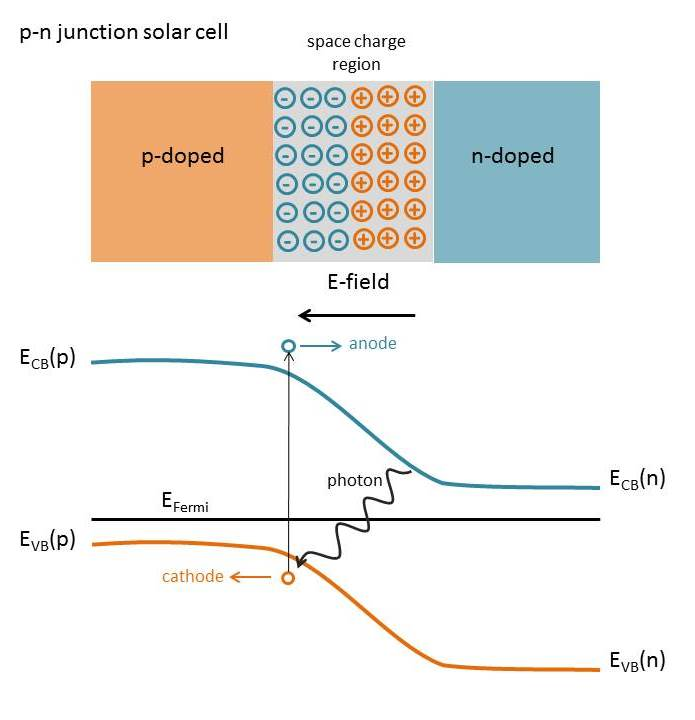
\includegraphics[scale=0.5]{pn-junction}
\caption{PN- Junction Diode}
\label{figc3h2} %% to refer use, \ref{}
\end{figure}

A pn-junction diode is formed by joining a p-type material with an n-type material. Now, at the junction of the diode the mobile electrons from the n region and the mobile holes from the p region of the diode drift by diffusion across the junction, leaving behind static positive charges and negative charges in the n region and p region of the diode respectively. These immobile charges create  a static electric field which opposes the diffusion of mobile electron and holes (also called charged carriers). The diffusion process continues till the electric field increases so much so that it restricts all further  diffusion of the charged carriers across the junction. This region of immobile charges at the junction is called the depletion region (depleted of mobile charged carriers). The width of the depletion region is about 1 $\mu \text{m} $ and the voltage across it is about 1 V; hence, electric field strength is about 10,000 V/cm. The Fig (\ref{diode12}) shows the symbol characteristics of a pn-junction diode.

\begin{figure}[H]
\centering
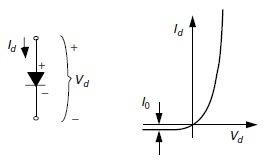
\includegraphics[scale=1]{diode1}
\caption{PN Juction Diode Symbol and Characteristics [5]}
\label{diode12} %% to refer use, \ref{}
\end{figure}

There are two modes of operation of a p-n junction diode. Firstly, the forward conduction mode, where an external positive voltage is applied across p-side and n-side (the external voltage cancels the effect of electric feild developed by the depletion region and allows for further diffusion reducing the width of the depletion region), in this mode the diode conducts very well offering least resistance. But, when a the voltage polarity across the pn-junction diode is reversed it blocks the flow of current offering maximum resistance, this mode of operation is called the reverse bias. Still a small amount of current flows due to thermally generated carriers, this current is called the reverse saturation current. The voltage-current characteristics for the pn-junction diode is described by the Shockley diode equation given by eq (\ref{diode}) 

\begin{equation}
\label{diode}
I_{d} = I_{0}( e^{qV_{d}/kT}-1)
\end{equation}\\
where,\\
$ I_{d} $ = Diode Current $ (A) $ \\
$ I_{0} $ = Reverse saturation current $ (A) $ \\
$ q $ = Electron charge $ (1.602\times10^{-19} C) $ \\
$ V_{d} $ = Voltage across diose terminals frm p-side to n-side $ (V) $ \\
$ k $ = Boltzman's constant $ (1.381\times10^{-23} J/K) $ \\

The Fig (\ref{d2}) shows the operation principle of a photovoltaic cell. When a pn-junction diode is exposed to sunlight, owing to the photo-electric effect photons of sunlight will be absorbed and electron-hole pairs will be formed.

\begin{figure}[H]
\centering
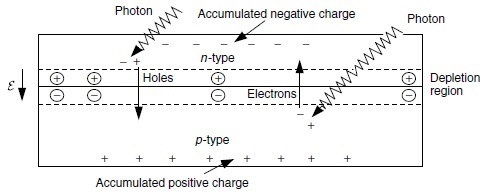
\includegraphics[scale=1]{pv8}
\caption{PN-Junction Diode as a Photovoltaic Cell [5]}
\label{d2} %% to refer use, \ref{}
\end{figure}

If these mobile charge carriers reach near the depletion layer, the electric field in the depletion layer will push the holes to the p-side and electrons to the n-side. Hence, holes will accumulate in the p-side and electrons in the n-side of the pn-junction diode. Now, if electrical contacts are attached to the pn-junction diode ends, conventional current will from p-side (electrons flow from the n-side) into the wire, through the load and back to the n-side, thus completing a circuit.\\

A simple model of a photovoltaic cell consists of a pn-junction diode in parallel with an ideal current source shown in Fig (\ref{p1}), where the ideal current source produces current in direct proportion to the amount of solar flux incident on it.

\begin{figure}[H]
\centering
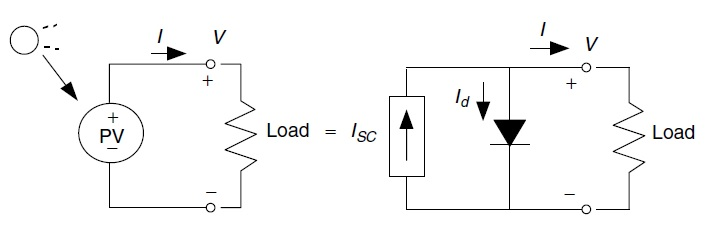
\includegraphics[scale=1]{pv9}
\caption{Simple Equivalent circuit of a Photovoltaic Cell [5]}
\label{p1} %% to refer use, \ref{}
\end{figure}

From Fig (\ref{pv9}) we can write the voltage and current equations for the PV cell as,

\begin{equation}
\label{pv1}
I = I_{SC}-I_{d}
\end{equation}\\
where,\\
$ I $ = Current output from PV Cell $ (A) $ \\
$ I_{SC} $ = Short circuit current of PV Cell $ (A) $ \\

Substituting the value of $I_{d}$ in above equation we get,

\begin{equation}
\label{pv2}
I = I_{SC}-I_{0} \left(e^{qV/kT}-1 \right )
\end{equation}

Where, $I_{SC}$ is the short circuit current, i.e. the current measured when the p-side and n-side are shorted, which means $V=0$, and $I$ is the load current.\\

Conversely, when the leads from the PV cell are kept open, no current flows i.e. $I=0$, the voltage measured is called as open-circuit voltage $(V_{OC})$, which is given by the following equation,

\begin{equation}
\label{pv3}
V_{OC} = \frac{kT}{q}\ln \left (\frac{I_{SC}}{I_{0}}+1\right )
\end{equation}\\
where,\\
$ V_{OC} $ = Open circuit voltage of PV Cell $ (V) $\\

The eq (\ref{pv2},\ref{pv3}) at $25^{\circ} \text{C}$ are given by the following equations,

\begin{equation}
\label{pv4}
I = I_{SC}-I_{0} \left(e^{38.9V}-1 \right )
\end{equation}

\begin{equation}
\label{pv5}
V_{OC} = 0.0257\ln \left (\frac{I_{SC}}{I_{0}}+1\right )
\end{equation} 



\subsection{PV Cell Model with Shunt Resistance}
\
\
\
\
A more accurate model of PV cell is developed when a resistance is added in parralel to the pn-junction diode as shown in Fig (\ref{fig3h4})

\begin{figure}[H]
\centering
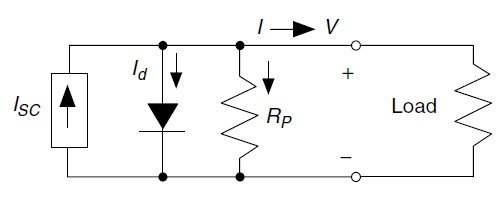
\includegraphics[scale=1]{PVmo}
\caption{PV Cell Model With Shunt Resistance [5]}
\label{figc3h4} %% to refer use, \ref{}
\end{figure}

This model describes the behaviour of a PV cell in a string of PV cell. If we consider that one of the PV cells in the string is shaded, then it will not produce current, moreover the pn-junction diode pertaining to that cell will be reverse biased and no current will not allow any flow of current. This will cause the entire current output from the string of PV cells to be reduced to zero, and no power is delivered to the load according to the simple equivalent model. But, in reality this is not the case and power though reduced in amount is delivered to the load even during shading. Hence, the voltage and current characteristics of a PV cell model with parallel resistance $R_{P}$ is given as follows,

\begin{equation}
\label{pv6}
I = (I_{SC}-I_{d})-\frac{V}{R_{P}}
\end{equation}\\
where,\\
$ V $ = Voltage at output of PV Cell $ (V) $ \\
$ R_{P} $ = Parallel resistance of the PV Cell $ (\Omega) $ 

\begin{figure}[H]
\centering
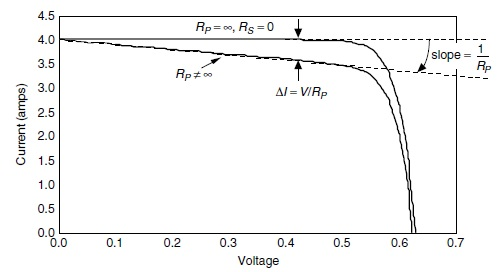
\includegraphics[scale=1]{pv1}
\caption{Effect of Parallel Resistance on I-V Curve [5]}
\label{figc3h111} %% to refer use, \ref{}
\end{figure}

The Fig (\ref{figc3h111]) shows the effect of parallel resistance on the I-V characteristics of the PV cell. It can be observed that the parallel resistance causes the load current for the simple model to be decreased by $V/R^{P}$.

\subsection{PV Cell Model with Series Resistance}
\
\
\
\
There is some intrinsic resistance of the semiconductor and also the contact resistance of the bond between the the wires and the cell leads. This resistance is called the series resistance ($R_{S}$), as it reduces the voltage availabe at the load terminals.
Hence, an accurate model of a PV cell should consinder $R_{S}$ as shown in Fig (\re{figc3h3})

\begin{figure}[H]
\centering
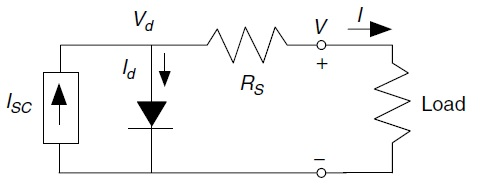
\includegraphics[scale=1]{PVmm}
\caption{PV Cell Model with Series Resistance [5]}
\label{figc3h3} %% to refer use, \ref{}
\end{figure}

The voltage and current characteristics of the PV cell with a series resistance are given by the following equations,

\begin{equation}
\label{pv7}
V_{d}=V+I.R_{S}
\end{equation}\\
where,\\
$ R_{S} $ = Series resistance of the PV Cell $ (\Omega) $ 

\begin{equation}
\label{pv8}
I = I_{SC}-I_{0} \left\{\text{exp}\left[\frac{q(V+I.R_{S})}{kT} \right]-1 \right\}
\end{equation}

\begin{figure}[H]
\centering
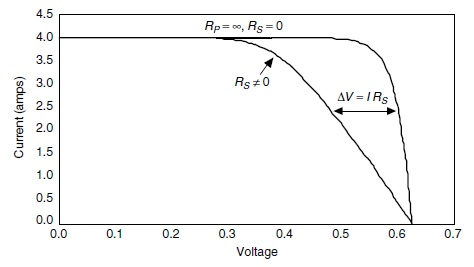
\includegraphics[scale=1]{pv2}
\caption{Effect of Series Resistance on I-V Curve [5]}
\label{figc3h222} %% to refer use, \ref{}
\end{figure}

The Fig (\ref{figc3h222}) shows the effect of series resistance on the I-V curve of the PV cell. It can be observed that the series resistance reduces the voltage available at the load by the factor of $IR_{S}$.

\subsection{Complete PV Cell Model}
\
\
\
\
The complete PV cell model as shown in Fig (\ref{figc3h333}) includes the both the parallel as well as the series resistance. This model of the PV cell is highly accurate.

\begin{figure}[H]
\centering
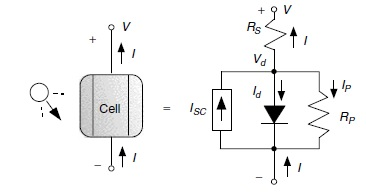
\includegraphics[scale=1]{pv3}
\caption{Complete Model of PV Cell [5]}
\label{figc3h333} %% to refer use, \ref{}
\end{figure}

The load current equation for this model is given by the following equation,

\begin{equation}
\label{pv10}
I_{SC}=I+I_{d}+I_{P}
\end{equation}\\
where,\\
$ I_{P} $ = Current in the parallel branch of the PV Cell $ (A) $\\ 

The effect of series resistance is given by the following equation,

\begin{equation}
\label{pv11}
V=V_{d}-IR_{S}
\end{equation}

The combined effect of the series and parallel resistances is given in the following equation, 

\begin{equation}
\label{pv9}
I = I_{SC}-I_{0} \left\{\text{exp}\left[\frac{q(V+I.R_{S})}{kT} \right]-1 \right\}-\left(\frac{V+I.R_{S}}{R_{P}}\right)
\end{equation}

\subsection{I-V Curve}
\
\
\
\
Fig (\ref{figc3h5}) shows the I-V curve of the PV cell. The I-V curve helps us identify the key parameters of the PV cell. On the horizontal axis we find open-circuit voltage $(V_{OC})$ when current is zero, and on the vertical axis we find the short-circuit current $(I_{SC})$ when the voltage is zero; at both these points the power delivered by the PV cell is zero as either voltage or current are zero $(P=VI)$.

\begin{figure}[H]
\centering
\includegraphics[scale=0.5]{PVivp [5]}
\caption{PV Cell I-V Curve}
\label{figc3h5} %% to refer use, \ref{}
\end{figure}

The maximum power delivered is obtained at the knee of the I-V curve, the point is called as the maximum power point (MPP). The voltage and current at the MPP are represented as $V_{m}$ and $I_{m}$. The I-V curve summarizes the entire performance characteristic of the PV cell. Any other point on the I-V curve is represented as $V_{R}$ and $I_{R}$.

\subsection{Effect of Insolation and Temperature on I-V Curve}
\
\
\
\
\
The Fig (\ref{figc3h6}) shows the PV cell curves for two different values of insolation. We observe that the short-circuit current is directly proportional to insolation, and it changes linearly with insolation. But, the open-circuit voltage is inversely proportional to the insolation, and it changes modestly with insolation as it follows a logarithmic relationship. Hence, as insolation increases the power output from the PV cell increases.

\begin{figure}[H]
\centering
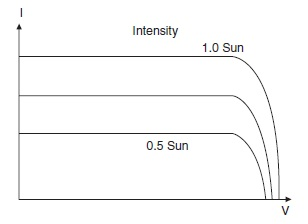
\includegraphics[scale=1]{PVinso}
\caption{Effect of Insolation on I-V Curve [5]}
\label{figc3h6} %% to refer use, \ref{}
\end{figure}

The Fig (\ref{figc3h7}) shows the PV cell curves for two different values of temperature. We observe that as temperature increases the open-circuit voltage decreases considerably, while the short-circuit current increases very slightly. Hence, the power output of PV cell increases on a clear and cold day. 

\begin{figure}[H]
\centering
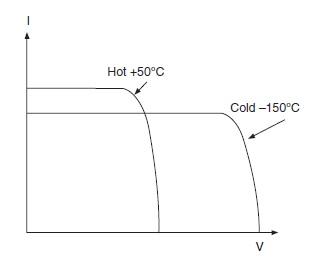
\includegraphics[scale=1]{PVtemp}
\caption{Effect of Temperature on I-V Curve [5]}
\label{figc3h7} %% to refer use, \ref{}
\end{figure}

The cell temperature depends not only on ambient temperature; but also on insolation as small fraction of insolation hitting the cell is converted to electricity, and the rest is converted to heat. Hence, manufacturers of the PV cells provide clients with a normal operating cell temperature (NOCT); it is the temperature in the cell when the ambient temperature is $20^{\circ} \text{C}}$, solar irradiance is $0.8 \  \text{kW/m}^{2}$, and windspeed is 1 m/s. This value helps in accounting the changes in the PV cell performance with temperature. The cell temperature can be calculated using the following equation, 

\begin{equation}
\label{tefpv}
T_{{cell}}=T_{{amb}}+\left(\frac{NOCT-20^{\circ}}{0.8}\right)
.\ S
\end{equation}

\newpage

\section{Cells, Modules and Arrays}
\
\
\
\
The individual cell with its small voltage of 0.5 V cannot be used alone for producing power for everyday applications. Hence, to increase the power output, a number of cells are connected together in series and parallel to form a module, which is encased in tough weather-resistant packages. Usually 36 cells are connected in series to give a module with voltage of 12 V and the number of parallel strings can be adjusted according to the amount of power to be generated from a module. Also, there are large modules with 72 cell connected in series giving a voltage of 72 V.

\begin{figure}[H]
\centering
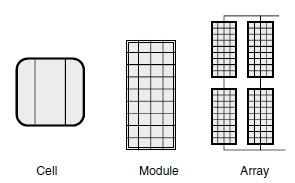
\includegraphics[scale=1]{pv4}
\caption{PV - Cell, Module and Array [5]}
\label{figc3h444} %% to refer use, \ref{}
\end{figure}

To increase the power generation capacity further, modules can be connected in series to increase voltage and a number of similar parallel strings can be connected to increase the current. Such a combination of modules is called as an array.

The eq (\ref{mod1}) gives the voltage equation for a module, where $n$ is the number of cells connected in series.

\begin{equation}
\label{mod1}
V_{{module}}=n(V_{d}-IR_{S})
\end{equation}\\
where,\\
$ V_{{module} $ = Total voltage of a PV Module $ (V) $ \\
$ n $ = Total number of PV Cells in one string in the PV Module  \\

From Fig (\ref{figc3h555}) we observe that as the number of cells in series in a module increase, the open-circuit voltage increases. But, the short-circuit current remains the same, hence the MPP has horizontal movement; and power output of the module increases

\begin{figure}[H]
\centering
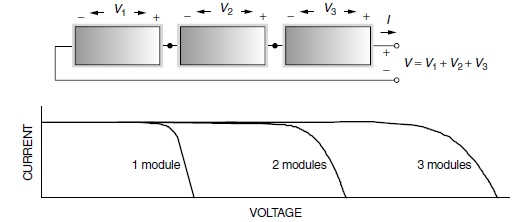
\includegraphics[scale=1]{pv5}
\caption{Effect of Series connected modules on I-V Curve [5]}
\label{figc3h555} %% to refer use, \ref{}
\end{figure}

The eq (\ref{mod2}) gives the current equation for a module, where $p$ is the number of strings in the module.

\begin{equation}
\label{mod2}
I_{{module}}=p(I_{SC}-I_{d}-I_{P})
\end{equation}\\
where,\\
$ I_{{module}} $ = Total current of the PV Module $ (A) $ \\
$ p $ = Total number of parallel strings of PV Cells in the PV Module\\

From Fig (\ref{figc3h666}) we observe that as the number of strings in a module increase, the short-circuit current increases. But, the open-circuit voltage remains the same, hence the MPP has a vertical movement; and power output of the module increases.

\begin{figure}[H]
\centering
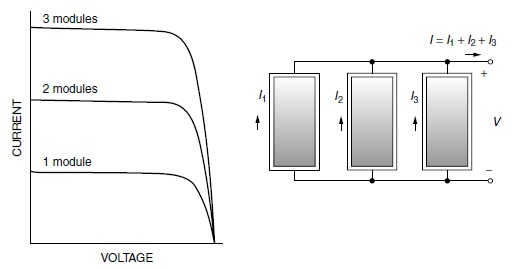
\includegraphics[scale=1]{pv6}
\caption{Effect of Parallel connected modules on I-V Curve [5]}
\label{figc3h666} %% to refer use, \ref{}
\end{figure}

\newpage

\section{Effect of Shading on PV Modules}
\
\
\
\
To understand the concept of shading in the PV cells let us consider the Fig (\ref{figc3h888}). It shows a string of $n$ cells, figure on the left shows condition when all the cells are in the sun. This will give us the usual behaviour of the PV module, where the major component of the current from the preceding cells will pass through the $I_{SC}$ current source branch.

\begin{figure}[H]
\centering
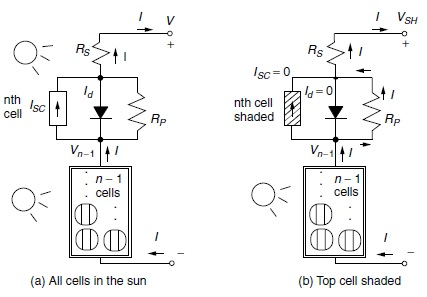
\includegraphics[scale=1]{shading1}
\caption{PV module with \textit{n} Cells - top cell in sun, or in shade [5]}
\label{figc3h888} %% to refer use, \ref{}
\end{figure}

But, the figure on the right shows the condition when one cell from the string is shaded (it does not produce current). Here we can see that the path taken by the current from the preceding cells in the string will have to pass through the branch of parallel resistance, which causes a large voltage drop as the value of parallel resistance is high. This drop in voltage reduces the power output of the module severely.\\

The output voltage $(V_SH)$ of the $n$ celled shaded module is given in the following equation,

\begin{equation}
\label{shade1}
V_{SH}=V_{n-1}-I(R_{P}+R_{S})
\end{equation}

Output voltage across $n-1$ cells $(V_{n-1})$ if $V$ is the output voltage of $n$ cells is given by, 

\begin{equation}
\label{shade2}
V_{n-1}=\left(\frac{n-1}{n}\right)V
\end{equation}\\
where,\\
$ n $ = Total number of cells ahaded $  $ \\
$ V_{n-1} $ = Output voltage across $ n-1 $ cells $ (V) $ \\
$ \triangledown V $ = Voltage drop caused by shaded cell $ (V}) $ 

Putting eq (\ref{shade2}) in eq (\ref{shade1}), we get;

\begin{equation}
\label{shade3}
V_{SH}=\left(\frac{n-1}{n}\right)V-I(R_{P}+R_{S})
\end{equation}\\
where,\\
$ V_{SH} $ = Output voltage of a $\text{n celled}$ shaded module $ (V) $ \\

Hence, the drop in voltage $(\triangledown)V$ at any given current $I$, caused by shaded cell is given by the following equation,

\begin{equation}
\label{shade4}
\triangledown V=\frac{V}{n}-I(R_{P}+R_{S})
\end{equation}\\
where,\\
$ \triangledown V $ = Voltage drop caused by shaded cell $ (V}) $ \\

The above equation can be modified as follows, as parallel resistance is very large as compared to the series resistance. Hence, neglecting the effect of series resistance, we get the following equation, 

\begin{equation}
\label{shade4}
\triangledown V=\frac{V}{n}-IR_{P}
\end{equation}

The Fig (\ref{figc3h999}) shows the comparison of I-V curves for an un-shaded and a shaded module. We can observe that in the module with shading both the short-circuit current and open-circuit voltage are reduced and the curve assumes a linear shape, which drastically reduces the power output from the module.

\begin{figure}[H]
\centering
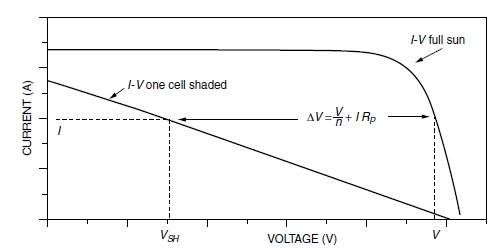
\includegraphics[scale=1]{shading2}
\caption{Effect of shading one cell in \textit{n} cell module [5]}
\label{figc3h999} %% to refer use, \ref{}
\end{figure}

\newpage

\subsection{Bypass Diode}
\
\
\
\
In order to overcome the problem of shading, bypass diodes are used as shown in Fig (\ref{figc3h100}). The figure on the left in Fig (\ref{figc3h100}) shows a PV cell which is un-shaded, here the bypass diode will be reverse biased as the PV ell produces reverse voltage across the bypass diode; hence, no current follow through the bypass diode when the cell is un-shaded.

\begin{figure}[H]
\centering
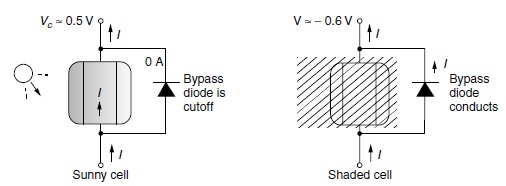
\includegraphics[scale=1]{bydiode1}
\caption{Mitigation of shading problem with Bypass Diode - In sunny cell bypass diode is cut-off, in shaded cell it conducts [5]}
\label{figc3h100} %% to refer use, \ref{}
\end{figure}

The figure in right in Fig (\ref{figc3h100}) shows a shaded PV cell with a bypass diode. As the cell is shaded the output voltage of the cell is reduced drastically, moreover the current from the preceding cells rather than passing through the parallel resistance of the shaded cell causing large voltage drop flows through the bypass diode as it gets forward biased. Hence, the bypass diode reduces the amount of voltage reduced due to shading(voltage drop in the bypass diode is about 0.5 V).

\begin{figure}[H]
\centering
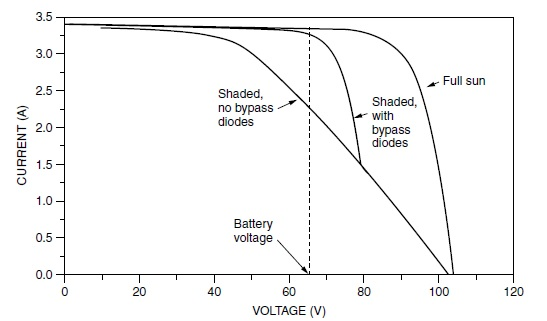
\includegraphics[scale=1]{bydiode2}
\caption{Effect of Bypass Diode on I-V Curve [5]}
\label{figc3h190} %% to refer use, \ref{}
\end{figure}

The Fig (\ref{figc3h190}) shows the comparison of I-V curves for shaded cell, un-shaded cell and shaded cell with bypass diode. We observe that the bypass diode improves the performance of the shaded cell by increasing the MPP point; however, it does not completely eliminate the effect of shading.

\subsection{Blocking Diode}
\
\
\
\
Blocking diodes as shown in Fig (\ref{figc3h200}) are connected at the top of each string of an array. The blocking diode will conduct only when the source of current is the string as it is in forward biased mode. But, when the string malfunctions or is shaded it acts as a load and draws current, the blocking diode becomes reverse biased and prevents any flow of current to the string. Hence a blocking diode helps improve the performance of a PV array.

\begin{figure}[H]
\centering
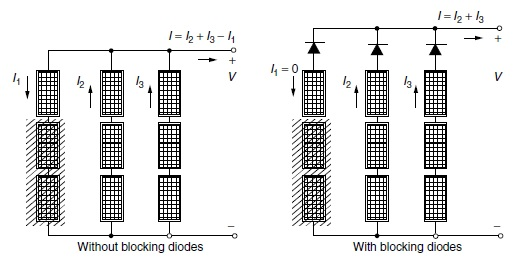
\includegraphics[scale=0.75]{bldiode1}
\caption{Blocking Diode prevents reverse flow of current through PV modules [5]}
\label{figc3h200} %% to refer use, \ref{}
\end{figure}

\newpage

\section{Results of PV-IV Curve App}
\
\
\
\
The Table (\ref{tabc3h1})gives the information of the different PV modules, which are used to simulate P-V and I-V curves from the PV-IV Curve App.

\begin{table}[htbp]
  \centering
  \caption{PV Module Information}
    \begin{tabular}{|l|c|c|c|c|}
    \hline
    \textbf{TYPE} & \textbf{Poly} & \textbf{Mono} & \textbf{Cdte} & \textbf{A-si} \bigstrut\\
    \hline
    \textbf{MAKE} & Lanco & Lanco & First Solar & Du-Pont \bigstrut\\
    \hline
    \textbf{Crys/TF} & Crys & Crys & TF & TF \bigstrut\\
    \hline
    \textbf{Pmpp (W)} & 235 & 250 & 85 & 107 \bigstrut\\
    \hline
    \textbf{Vmpp (V)} & 29.56 & 31.15 & 46.4 & 74 \bigstrut\\
    \hline
    \textbf{Impp (A)} & 7.95 & 8.034 & 1.83 & 1.44 \bigstrut\\
    \hline
    \textbf{Voc (V)} & 37.17 & 38.04 & 60.5 & 99 \bigstrut\\
    \hline
    \textbf{Isc (A)} & 8.4 & 8.712 & 1.94 & 1.81 \bigstrut\\
    \hline
    \textbf{Kv} & -0.31 & -0.33 & -0.27 & -0.3 \bigstrut\\
    \hline
    \textbf{Ki} & 0.06 & 0.036 & 0.04 & 0.09 \bigstrut\\
    \hline
    \textbf{Kp} & -0.43 & -0.47 & -0.25 & -0.25 \bigstrut\\
    \hline
    \end{tabular}%
  \label{tabc3h1}%
\end{table}%
\\
Where Crys-Crystalline, TF-Thin Film, mmp-Maximum Power Point, oc-Open Circuit, sc-Short Circuit, P-Power, V-Voltage, I-Current and Kv, Ki, Kp are the temperature co-efficients of voltage, current and power respectively.\\

The PV and IV curves are plotted at different temperatures (-25, 0, 25, 50 and 75 ºC) and different irradiances ( 200, 400, 600, 800 and 1000 W/m^{2}) are as follows,

\begin{figure}[H]
\centering
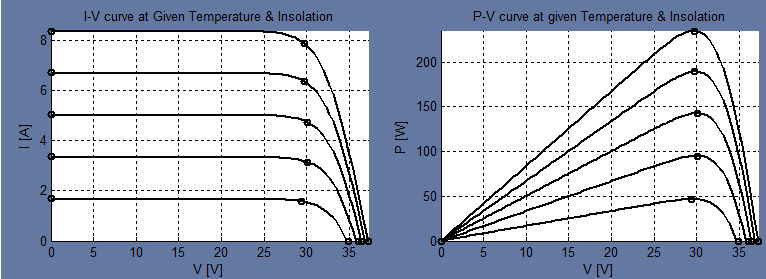
\includegraphics[scale=0.5]{Poly_Irradiance}
\caption{Polycrystalline Solar PV module I-V and P-V Curves at different Irradiances}
\label{figc3h15} %% to refer use, \ref{}
\end{figure}

\begin{figure}[H]
\centering
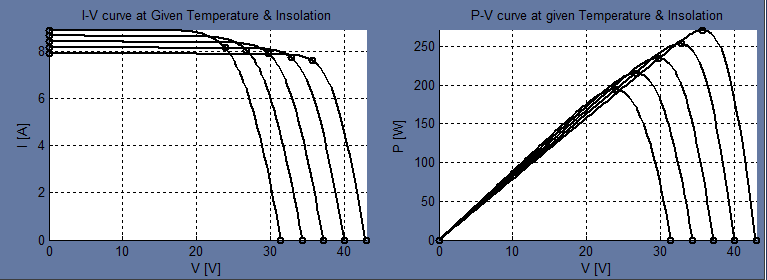
\includegraphics[scale=0.5]{Poly_Temperature}
\caption{Polycrystalline Solar PV module I-V and P-V Curves at different Temperatures}
\label{figc3h16} %% to refer use, \ref{}
\end{figure}

\begin{figure}[H]
\centering
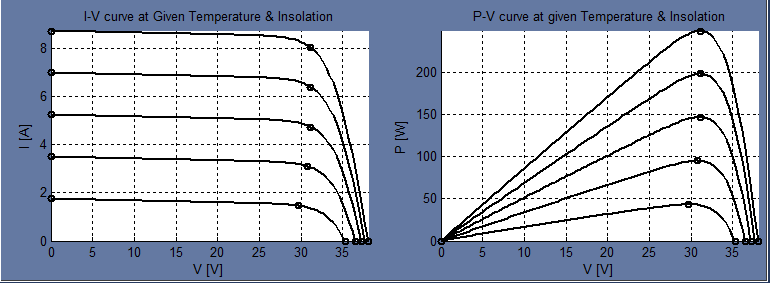
\includegraphics[scale=0.5]{Mono_Irradiance}
\caption{Monocrystalline Solar PV module I-V and P-V Curves at different Irradiances}
\label{figc3h17} %% to refer use, \ref{}
\end{figure}

\begin{figure}[H]
\centering
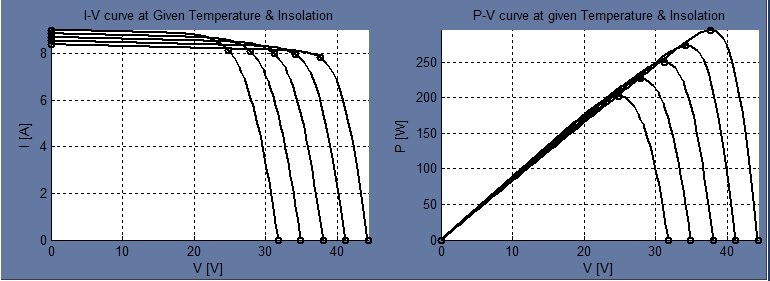
\includegraphics[scale=0.5]{Mono_Temperature}
\caption{Monocrystalline Solar PV module I-V and P-V Curves at different Temperatures}
\label{figc3h18} %% to refer use, \ref{}
\end{figure}

\begin{figure}[H]
\centering
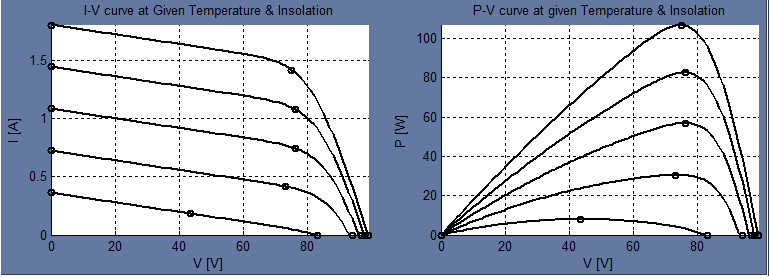
\includegraphics[scale=0.5]{A-si_Irradiance}
\caption{A-Si Thin Film Solar PV module I-V and P-V Curves at different Irradiances}
\label{figc3h19} %% to refer use, \ref{}
\end{figure}

\begin{figure}[H]
\centering
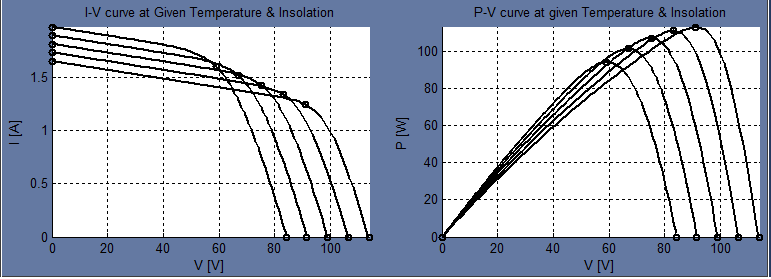
\includegraphics[scale=0.5]{A-si_Temperature}
\caption{A-Si Thin Film Solar PV module I-V and P-V Curves at different Temperatures}
\label{figc3h20} %% to refer use, \ref{}
\end{figure}

\begin{figure}[H]
\centering
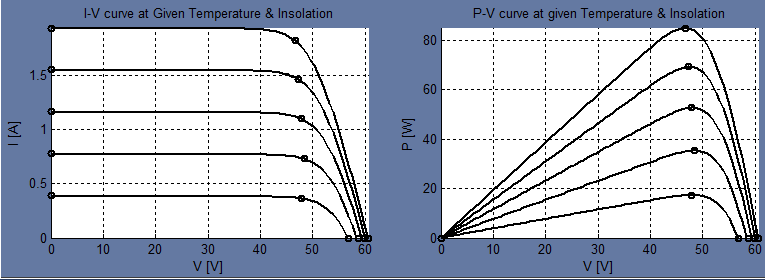
\includegraphics[scale=0.5]{CDTE_Irradiance}
\caption{CDTE Thin Film Solar PV module I-V and P-V Curves at different Irradiances}
\label{figc3h21} %% to refer use, \ref{}
\end{figure}

\begin{figure}[H]
\centering
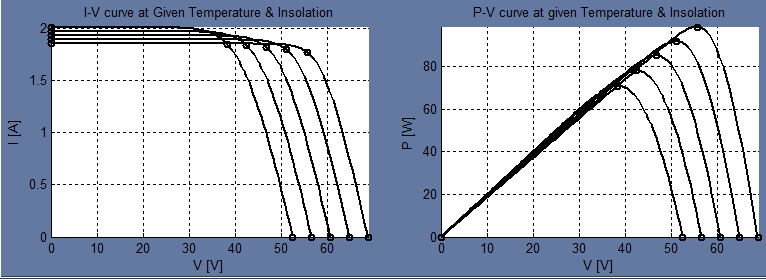
\includegraphics[scale=0.5]{CDTE_Temperature}
\caption{CDTE Thin Film Solar PV module I-V and P-V Curves at different Temperatures}
\label{figc3h22} %% to refer use, \ref{}
\end{figure}
The effect of decreasing irradiance with temperature at kept constant at 25ºC can be observed in Fig (\ref{figc3h15}, \ref{figc3h17}, \ref{figc3h19}, \ref{figc3h21}). It is clearly seen that the photovoltaic module current output and power are directly proportional to the irradiance level, however the module voltage increases by very small values with decreasing irradiance levels. This concurs with the theory that module current is a direct function of the solar irradiance.\\

The effect of increasing temperature with irradiance level kept constant at 1000 W/m2 can be observed in Fig (\ref{figc3h16}, \ref{figc3h18}, \ref{figc3h20}, \ref{figc3h22}). It is clearly seen that the module voltage and power output are inversely proportional to the temperature, however the module current increases very slightly with increase in temperature. This concurs with theory that diode voltage is inversely proportional to temperature.

\begin{figure}[H]
\centering
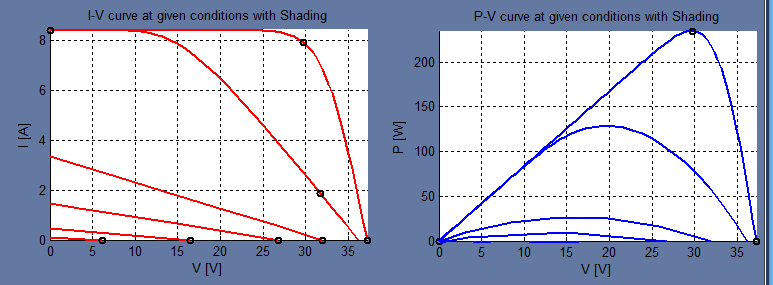
\includegraphics[scale=0.5]{Poly_Shading_WithoutByPassDiode}
\caption{Polycrystalline Solar PV moduleP-V and I-V curves for Shading without Bypass Diode and at different number of shaded cells}
\label{figc3h23} %% to refer use, \ref{}
\end{figure}

\begin{figure}[H]
\centering
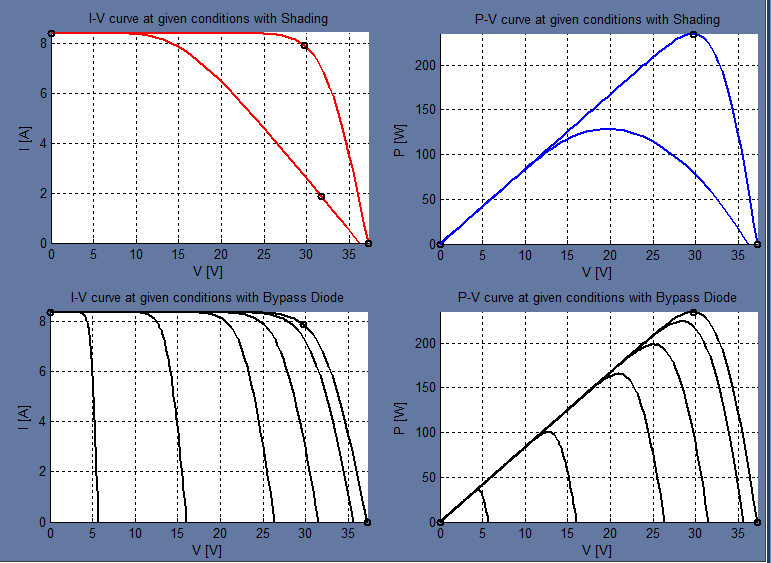
\includegraphics[scale=0.5]{Poly_Shading_With_ByPassDiode}
\caption{Polycrystalline Solar PV moduleP-V and I-V curves for Shading with Bypass Diode and at different number of shaded cells}
\label{figc3h24} %% to refer use, \ref{}
\end{figure}

In Fig (\ref{figc3h23}) we can observe that as the number of single cells within a module being shaded increase, both the PV and IV curves start becoming flat. Hence, shading of even a single cell almost reduces the module power by half and this can be attributed to the voltage loss in the series and parallel equivalent resistances due to the flow of the module output current.\\

To mitigate the shading effect, bypass diodes are used, which allow for alternative path to the current to flow which would have otherwise flowed through Rp and Rs causing large voltage drops, which consequently causes large reductions in output power. Ideally for the best shading effect mitigation, each cell within a module should be supplied with its own bypass diode, but as this would be escalate the cost and manufacturing complexity; hence optimal number of cell per bypass diodes have to selected. In Fig (\ref{figc3h24}) it can be observed that as the number of cell per bypass diode increase the performance of the module deteriorates.\\

\newpage

\section{Variables Affecting Solar PV Cell Output}
\
\
\
\
From the discussions in the previous sections, it is clear that the performance of a PV Cell depends on the following four variable;

\begin{enumerate}
\item Insolation
\item Temperature
\item Wind Speed
\item Cloud Cover
\end{enumerate}

The Fig (\ref{mfigc3h1}) shows pictures of some instruments which help in measuring the above mentioned variables.

\begin{figure}[H]
    \centering
    \begin{subfigure}[b]{0.45\textwidth}
       \centering
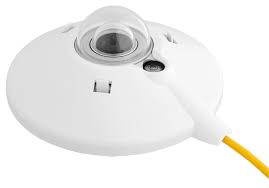
\includegraphics[scale=0.5]{Pyranometer}
\caption{Pyranometer}
\label{figc3h8}
    \end{subfigure}
    \hfill%% Fill Horizontal Space between two Figures
        \begin{subfigure}[b]{0.45\textwidth}
       \centering
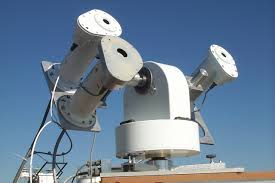
\includegraphics[scale=0.5]{Pyrheliometer}
\caption{Pyrheliometer}
\label{figc3h9} %% to refer use, \ref{}
    \end{subfigure}
    \caption{}
    \label{}
\end{figure} 
   

\begin{figure}[H]
    \centering
    \begin{subfigure}[b]{0.45\textwidth}
\centering
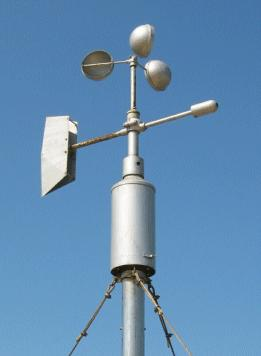
\includegraphics[scale=0.5]{Anemometer}
\caption{Anemometer}
\label{figc3h10} %% to refer use, \ref{}
    \end{subfigure}
    \hfill%% Fill Horizontal Space between two Figures
        \begin{subfigure}[b]{0.45\textwidth}
\centering
\includegraphics[scale=0.5]{Temperature}
\caption{TEmperature Sensor}
\label{figc3h11} %% to refer use, \ref{}
    \end{subfigure}
    \caption{Weather Variables Measurement Instruments}
    \label{mfigc3h1}
\end{figure}  

The Fig (\ref{figc3h8}) shows a Pyranometer, it mmeasures the Global Horizontal Irradiance. The Fig (\ref{figc3h9}) shows a Pyrheliometer, it measures the Direct Beam Irradiance of the sun. The Fig (\ref{figc3h10}) shows an Anemometer, which measures the wind speed. The Fig (\ref{figc3h11}) shows a temperature sensor. Also, there is a sky imager which can measure the cloud cover.

\section{PV Cell Technologies}
\
\
\
\
There are majorly three PV technologies, Mono-Crysalline, Poly-Crystalline and Thin Film which are commercially widely used in Solar PV Plants.

\subsection{Mono-Crystalline PV}

\begin{figure}[H]
\centering
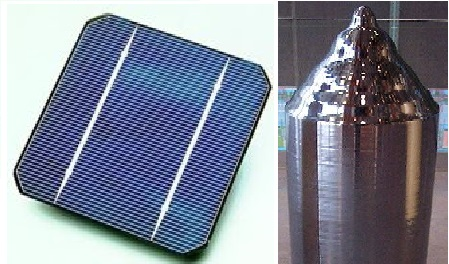
\includegraphics[scale=2]{PVmono}
\caption{Mono-Crystalline Cell and its Crystal}
\label{figc3h12} %% to refer use, \ref{}
\end{figure}

It is manufactured by slicing thin wafers from a single long Silicon crystal rod (shown in the figure at the right of Fig (\ref{figc3h12} ) using Czochralski process. It is the most expensive of the three technologies. It has an efficiency of 15-20\%, and has the highest density of power production (area/power is lowest). It has a market share of 36%.

\subsection{Poly-Crystalline PV}

\begin{figure}[H]
\centering
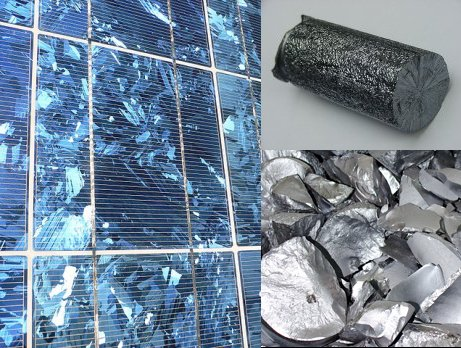
\includegraphics[scale=0.5]{PVPoly}
\caption{Poly-Crystalline Cell and its Crystal}
\label{figc3h13} %% to refer use, \ref{}
\end{figure}

It is manufactured from the metallurgical grade silicon (shown in the figure at the right of Fig \ref{figc3h13} ) by a chemical process, called as Siemens process. It is the moderately priced. It has an efficiency of 13-16\%, and has the moderate density of power production (area/power is lower than Mono-Crystalline). 

\subsection{Thin Film PV}

\begin{figure}[H]
\centering
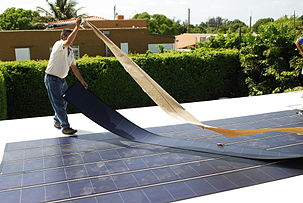
\includegraphics[scale=2.5]{PVthin}
\caption{Thin Film Sheet}
\label{figc3h14} %% to refer use, \ref{}
\end{figure}

It is manufactured by depositing one or more thin layes of PV material on a substrate such as glass, plastic or metals. The  Fig (\ref{figc3h13}) shows the Thin Film PV sheet. It is the least expensive of the three technologies. But, has has an efficiency of 7-13\%, and has the lowest density of power production (area/power is lowest). 